\documentclass[a4paper,10pt]{article}

%\usepackage[utf8]{inputenc}
\usepackage{graphicx}
\usepackage{url}
\usepackage{float}
\usepackage{times}
\usepackage{multirow}
\usepackage{listings}
\usepackage{times}
\usepackage{paralist}
\usepackage{epsfig}
\usepackage{subfigure}
\usepackage[hypertex]{hyperref}
\usepackage{subfigure}
\usepackage{color}
\usepackage{ifpdf}

\newcommand{\I}[1]{\textit{#1}}
\newcommand{\B}[1]{\textbf{#1}}
\newcommand{\BI}[1]{\textbf{\textit{#1}}}
\newcommand{\T}[1]{\texttt{#1}}
\newcommand{\dctf}{dC$_{25}$ }
\newcommand{\dctfnsp}{dC$_{25}$}
\newcommand{\atf}{A$_{25}$ }
\newcommand{\dco}{dC$_{1}$ }
\newcommand{\atfnsp}{A$_{25}$}
\newcommand{\dconsp}{dC$_{1}$}
\newcommand{\aonsp}{A$_{1}$}
\newcommand{\ao}{A$_{1}$ }
\newcommand{\ato}{A$_{1}$ }
\newcommand{\ahl}{$\alpha$HL }
\newcommand{\ahlnsp}{$\alpha$HL}
\newcommand{\prim}{$^{\prime}$ }
\newcommand{\primnsp}{$^{\prime}$}


\pdfpagewidth 8.5in
\pdfpageheight 11in 

\setlength\topmargin{0in}
\setlength\headheight{0in}
\setlength\headsep{0in}
\setlength\textheight{9in}
\setlength\textwidth{6.5in}
\setlength\oddsidemargin{0in}
\setlength\evensidemargin{0in}
\setlength\parindent{0.1in}
\setlength\parskip{0.25em}

\ifpdf
 \DeclareGraphicsExtensions{.pdf, .jpg}
\else
 \DeclareGraphicsExtensions{.eps, .ps}
\fi

\newcommand{\jha}[1]{ {\textcolor{red} { ***Jha: #1 }}}

\begin{document}
\title{\large Investigating Scale-Out Performance of 
Loosely-Coupled Simulations Using Multiple Distributed Resources on the TeraGrid. Understanding the Energetics and Conformational Configurations of Nucleic Acids}

\author{Principal Investigaor: Shantenu Jha$^{1,2}$ \\ Co-Principal Investigaor: Joohyun Kim$^{1}$ \\ Co-Principal Investigaor: Yaakoub El Khamra$^{3}$\\\
   \small{\emph{$^{1}$Center for Computation \& Technology, Louisiana State University, Baton Rouge, 
USA}}
\\
  \small{\emph{$^{2}$Department of Computer Science, Louisiana State
      University, Baton Rouge, USA}}
\\
  \small{\emph{$^{3}$Texas Advanced Computing Center TACC, University of Texas, Austin, USA}}}

\newif\ifdraft
\drafttrue
\ifdraft
\newcommand{\amnote}[1]{ {\textcolor{magenta} { ***AM: #1c }}}
\newcommand{\jhanote}[1]{ {\textcolor{red} { ***SJ: #1 }}}
\newcommand{\michaelnote}[1]{ {\textcolor{blue} { ***MM: #1 }}}
\else
\newcommand{\amnote}[1]{}
\newcommand{\jhanote}[1]{}
\newcommand{\michaelnote}[1]{ {\textcolor{blue} { ***MM: #1 }}}
\fi


\date{15 July 2009}

\maketitle

\subsection*{Summary:} Over the past two years, we have been involved in a wide range of computational science and computer science projects, requiring a few groups to use multiple resources on the TeraGrid concurrently (for loosely-coupled simulations). In this proposal we request 2.0M SUs for three distinct projects: (i) understanding translocation of nucleic acid in $\alpha$-Hemolysin protein pores; (ii) conformational switching of S-box riboswitch and, (iii) for developing and enhancing the understanding of distributed applications and testing the {\it scale-out } performance of a range of applications. The projects for which computer time is being requested are all funded projects -- some at the national level, and some by local resources; those that are not funded by NSF/NIH form the basis for upcoming significant NSF/NIH proposals.  Additionally, the request for 2.0M SUs in this proposal is based upon the projected science problems as outlined below as well as a proven track record of {\it successfully} utilising more than 1.2M SUs in the last year (large allocation of 900,000 SUs on Queen Bee, several small DAC award and multiple concurrent starter awards).

% \jhanote{Yaakoub, please determine the correct units?  Is it SUs, NU or some other metric. Thanks.}

% \jhanote{Issues: Final Number of CPU Hrs?  Which resource? What component should be roaming?}

\section{Project 1: Nucleic Acid Translocation through Alpha-Hemolysic Protein Nanopore}

The translocation of polynucleotides across membranes is a fundamental
biological process, with important technological and medical
relevance.  The translocation process is complex and is influenced by
a range of factors including the diameter and inner surface of the
pore, the secondary structure of the polymer, and interactions between
polymer and protein. We have performed non-equilibrium constant
velocity-steered molecular dynamics (cv-SMD) simulations of nucleic
acid molecule translocation through the protein nanopore
$\alpha$-hemolysin (\ref{fig:edge}) and used Jarzynski's
identity~\cite{jarz} to determine the associated free
energy profiles. Constant velocity-steered molecular
dynamics~\cite{namd} (cv-SMD) is a type of non-equilibrium
simulation that connects an atom or center of mass of a group of atoms
via a harmonic spring (governed by a force or spring constant, $k$) to
a constraint position which is moved at constant velocity. Cv-SMD has
the advantage of a well defined wall-clock and simulated time-frame
for a given translocation distance, allowing the induction of
high-speed translocation in a consistent manner.

\begin{figure}[!h]
  \begin{center}
    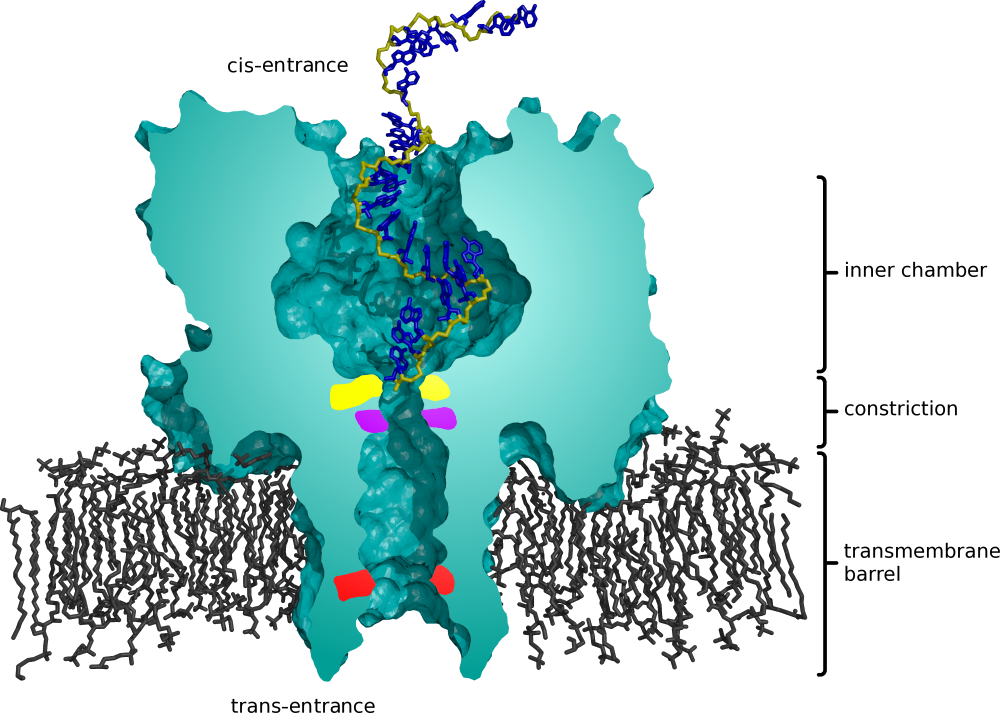
\includegraphics[width=5.0in]{ahl_labelled13}
  \end{center}
  \caption{Figure representing the starting configuration of a 3\prim
led \atf translocation simulation. The heptameric protein pore \ahl
(green) is inserted into a lipid bilayer (black). Features of the
translocating molecule include the backbone of \atf (dark yellow) and
the nucleic acid bases (blue). The $trans$-entrance is at the bottom
of the pore; taking the $trans$-entrance of \ahl as a reference point
at 0~{\AA}, other notable features include protein residue Leu-135 at
13~{\AA} (red), Met-113 at 43~{\AA} (pink), Lys-147 at 45~{\AA} (light
yellow), and the $cis$-entrance at the top of the protein at
95~{\AA}. The $cis$-entrance is 28~{\AA} in diameter, the wide section
of the pore running from the $cis$-entrance to residue Lys-147 is
termed the inner chamber and is up to 46~{\AA} wide. The constriction
marked by residues Lys-147 and Met-113 is 14~{\AA} wide, while the
transmembrane barrel runs from the constriction to the
$trans$-entrance and is around 20~{\AA} wide; the $trans$-entrance is
24~{\AA} wide. The C3\prim carbon atom of the 3\prim end residue of
\atf is aligned with the center of mass of the C$_{\alpha}$ atoms of
protein residue 111, which lies at the mouth of the constriction, just
above residue Lys-147. For the sake of clarity, water molecules,
sodium and chloride ions are not displayed (they are found along the
entire length of the pore).}
  \label{fig:edge}
\end{figure} 


With this approach we have been able to explain the observed
differences in experimental translocation time through the nanopore
between polyadenosine and polydeoxycytidine. Poly(A) and poly(dC)
molecules of 100-200 bases in length exhibit a 20-fold difference in
translocation time through \ahl in SCCR
experiments~\cite{akeson}. The translocation of both 25 base
polynucleotides and single nucleotides through $\alpha$-hemolysin has
been investigated. An example of our results which qualitatively agree
with experimental finding can be seen in~\ref{full_trans_local}. These
simulations are computationally intensive as they employ models with
atomistic level resolution; in addition to their size, these systems
are challenging to study due to the time-scales of translocation of
large asymmetric molecules. Our simulations have provided insight into
the role of the interactions between the nucleic acid molecules and
the protein-pore. Mutated protein-pores have provided confirmation of
residue-specific interactions between nucleotides and the
protein-pore. By harnessing such molecular dynamics simulations, we
have gained new physical insight into the translocation process. 

This work has been accepted for publication and will be imminently published in the Journal of Chemical Theory and Computation (H. Martin, S. Jha, S. Howorka, P. Coveney, Determination of Free Energy Profiles for the Translocation of Polynucleotides through $\alpha$-Hemolysin Nanopores using Non-Equilibrium Molecular Dynamics Simulations). In the JCTC paper we pushed cv-SMD to new limits, testing the validity of the method for a larger translocating molecule and higher atom count system than ever previously attempted at such relatively low pulling speeds. In the paper we showed that an interaction between a positively charged lysine residue of the pore interior and the negatively charged nucleotide phosphate groups give rise to peaks in the free energy profiles. We also highlighted key ion interactions that play a role in these phospate-lysine interactions, pointing to important considerations for future computational scientists to consider.


\begin{figure}[!h]
  \begin{center}
    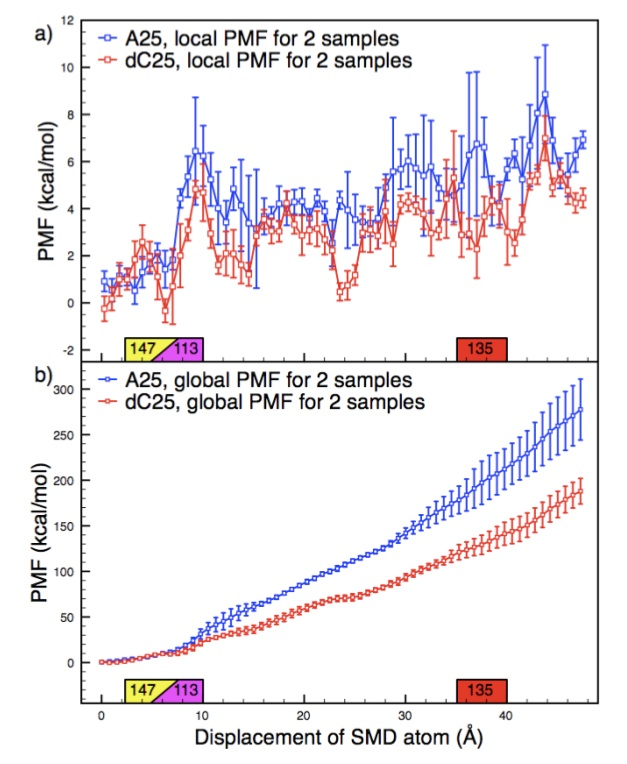
\includegraphics[width=4.0in]{full_trans_1every3_b}
  \end{center}
    \caption{a) Local free energy profiles of \atf and \dctf
translocation from the top of the constriction to the bottom of the
$trans$-entrance; each profile was derived from two samples. Labelled
along the $x$-axis are protein residues Met-147, Lys-113, and Leu-135.
The residue labels span 5~{\AA} from when the pulled atom to first
phosphate atom passes the labelled residue. The plot shows poor
separation of \atf and \dctf when considering the error bars, though a
general trend where \atf has a higher free energy profile than \dctf
is observed. An overall increase in the free energy profile is
observed from left to right, which is expected as more residues enter
the confining dimensions of the constriction and transmembrane
barrel. b) Global free energy profile of \atf and \dctf
translocation from the top of the constriction to the bottom of the
trans-entrance; each profile was derived from two samples. The plot
shows good discrimination of \atf and \dctf beyond the error bars. The
error bars indicate greater sample-to-sample variation around the
constriction and towards the end of the transmembrane barrel, which
may indicate non-steric contributions at these
points.}
  \label{full_trans_local}
\end{figure}

The high-level scientific objective for this project is to compute free energy profiles of the translocation process of DNA along the vertical axis of a transmembrane protein pore buried in a lipid membrane bilayer. This is a project that has been ongoing for nearly three years % (which was initiated before my transition to LSU),
and has consumed a total of about 6M SUs so far. The work that has been published so far covers relatively low sampled instances of nucleotide and single nucleotide translocation through wild type and mutated protein pores, yielding good results and has established the groundwork for further publications. The project uses the parallel MD code NAMD and as also led to a grid-enabled version of NAMD developed by us to perform steered MD simulations including the capability to connect to distributed haptic devices. This work is currently funded by the UK's EPSRC (equivalent to the US NSF). % Current and near-future work, also forms the basis of a joint US-UK submission to the NSF (in collaboration with Prof.'s Zuzanna Siwy (UC-Irvine) and Stefan Howorka (London)).

Currently and in the near future we will be expanding the sampling of
all the explored systems to yield solid and consistent results. The
published set of data represents 2 to 6 samples per free energy
profile, we are now looking to expand this to 16 samples for each
system investigated (see Table~\ref{table:systems}). This will allow
us to confidently compare the results to means of translocation other
than cv-SMD. One such method that we are currently attempting to apply
to the system is using an Adaptive Biasing Force (ABF). Here the
translocating atom (and thus the attached molecule) is moved via a
biasing force which acts to overcome energy barriers in order to
translocate along a reaction coordinate. The biasing force adapts to
the free energy landscape on-the-fly, which allows less control over
the translocation speed compared to cv-SMD, but a trivially expanded
degree of sampling for the free energy profile, given suitable
supercomputing resources. The JCTC paper served to highlight important
differences between the conditions under a cv-SMD simulation and SCCR
experiments, and highlighted the general issues that arise when
inducing translocation using cv-SMD. For instance, due to the
translocation force acting on the front of the polynucleotide instead
of the whole molecule, conformational relaxation forces were not
permitted time to maintain a realistic polynucleotide conformation,
even at our slowest pulling conditions. By translocating using ABF,
the process will be much closer to equilibrium andso may avoid this
short-coming of cv-SMD. Therefore, by performing the same process
using ABF we will be able to evaluate both methods, and present our
findings to the field.

\begin{table}[!h]
\begin{center}
  \caption{The translocation molecules and pore types
to be simulated. `Wild Type' indicates \ahl with no mutated residues;
'Mutant' indicates \ahl mutant L147M.\newline  
}
\label{table:systems}
\begin{tabular}{| c | c | c | c | c | c | c |}
\hline
Pulling & System & \ahl Type & Nucleotide & Nucleotides & Samples &
SUs \\
Method & Name &  & Base &  & Performed & required \\
\hline
cv-SMD & \aonsp-WT & Wild Type & Adenine & 1 & 16/16 & - \\
cv-SMD & \atfnsp-WT & Wild Type & Adenine & 25 & 16/16 & - \\
cv-SMD & \dconsp-WT & Wild Type & Deoxycytosine & 1 & 16/16 & - \\
cv-SMD & \dctfnsp-WT & Wild Type & Deoxycytosine & 25 & 14/16 & 25K\\
cv-SMD & \aonsp-Mut & Mutant & Adenine & 1 & 2/16 & 200K \\
cv-SMD & \atfnsp-Mut & Mutant & Adenine & 25 & 2/16 & 200K \\
cv-SMD & \dconsp-Mut & Mutant & Deoxycytosine & 1 & 2/16 & 200K \\
cv-SMD & \dctfnsp-Mut & Mutant & Deoxycytosine & 25 & 2/16 & 200K \\
ABF & \atfnsp-ABF & Wild Type & Adenine & 25 & N/A & 0.5M \\
ABF & \dctfnsp-ABF & Wild Type & Deoxycytosine & 25 & N/A & 0.5M \\
\hline
\end{tabular}
\end{center}
\end{table}


The increased cv-SMD sampling has so far consumed about 3.5M SUs (to be contrasted with 6M for the overall project) and about 
2M more are required to finish sampling the remaining systems (specifically, translocation through mutated \ahl pores).  The ABF simulations should consume between 1 and 2M SUs, though the precise number is difficult to predict due to the nature of ABF. If necessary, the degree of sampling and the length of translocation can be adjusted to work within a given SU allocation. Therefore we ask for 1M SUs to be allocated to us for use on this project.

%\begin{table}[!h]
%\begin{center}
%  \caption{The translocation molecules and pore types
%to be simulated. `Wild Type' indicates \ahl with no mutated residues,
%'Mutant' indicates \ahl mutant L147M.\newline  \jhanote{Hugh: Can you add another column where you estimate the number of CPU hours you'll require. I'm tryiing to make the number of 2M not seem to be arrived at in
%a coarse-grained fashion, hence want some details}}
%\label{table:systems}
%\begin{tabular}{| c | c | c | c | c | c |}
%\hline
%Pulling & System & \ahl Type & Nucleotide & Nucleotides & Samples \\
%Method & Name &  & Base &  & Performed \\
%\hline
%cv-SMD & \aonsp-WT & Wild Type & Adenine & 1 & 16/16 \\
%cv-SMD & \atfnsp-WT & Wild Type & Adenine & 25 & 16/16 \\
%cv-SMD & \dconsp-WT & Wild Type & Deoxycytosine & 1 & 16/16 \\
%cv-SMD & \dctfnsp-WT & Wild Type & Deoxycytosine & 25 & 14/16 \\
%cv-SMD & \aonsp-Mut & Mutant & Adenine & 1 & 2/16 \\
%cv-SMD & \atfnsp-Mut & Mutant & Adenine & 25 & 2/16 \\
%cv-SMD & \dconsp-Mut & Mutant & Deoxycytosine & 1 & 2/16 \\
%cv-SMD & \dctfnsp-Mut & Mutant & Deoxycytosine & 25 & 2/16 \\
%ABF & \atfnsp-ABF & Wild Type & Adenine & 25 & N/A \\
%ABF & \dctfnsp-ABF & Wild Type & Deoxycytosine & 25 & N/A \\
%\hline
%\end{tabular}
%\end{center}
%\end{table}

\subsection*{Project 2: Computational Study of non-coding Functional RNAs: Binding mechanism of Riboswitches}

%Increasing attention has focused on targeting RNAs for drug design~\cite{foloppe}. 

While increasing evidences have indicated a critical role of structured nc-RNAs in gene regulations of both transcription and translation levels, suggesting the potential of targeting RNA for drug
design~\cite{foloppe} and bioengineering applications, an understanding of the interactions of nc-RNAs with other molecules such as small metabolite, proteins, and RNAs remains as fundamental challenges.  The roles of computational means, therefore, are critical component for holistic understanding on dynamics and interactions of RNAs.  

Among nc-RNAs, our primary targets are riboswitch RNAs. Riboswitches are regulatory RNAs that control the expression of downstream genes. Small metabolite 
molecules, such as amino acids, nucleotides, coenzymes etc., can bind to riboswitches as effectors in  vivo~\cite{mandal}. 
In our recent research efforts, the S-box riboswitch (also called SAM-I riboswitch), one member of the riboswitch family that
regulates the metabolism of sulfur and methionine, has been extensively investigated with atomistic simulations.  This riboswitch choose alternative conformation depending on binding of a SAM .  When S-adenosylmethionine (SAM) is bound, the
aptamer domain forms anti-anti-terminator (AAT) conformation,
which turns off the downstream genes by forming the terminator (T). Otherwise, the anti-terminator (AT) is formed prohibiting the T element formation for continuing transcription process (Figure 3a)~\cite{brooke}. Although the 
structure of the s-box in the anti-anti-terminator (AAT) conformation has been solved via X-ray 
crystallography, it is just a static view of how SAM binds to the s-box.  Using extensive all-atom simulations, we became to propose a novel binding mechanism of the SAM-I riboswitch with a SAM in which the role of entropic barrier for the AAT formation as well as the role of $Mg^2+$ specifically bound in the tertiary core structure.  Our obtained results are contained in the paper submitted to the journal, Nucleic Acid Research.  The paper is now under the review.~\cite{SAM-I-NAR2009}  Continuing our efforts, the goal of this study is to probe 
the dynamic interactions between the s-box riboswitch and SAM at the nanoscale and to explore 
determinants for the specificity. In particular, encouraged by our initial results, we aim to extend our strategy, combining MD and statistical analysis, for i) other constructs of SAM-I that differ from each other in potentially different secondary structures and tertiary interactions, ii) different sequences in SAM-I family, and iii) other SAM riboswiches (SAM-II and SAM-III) for which X-ray structures are known.  To estimate binding affinity, we use MM-PBSA but also expect novel theoretical developments considering the challenges arising from strong electrostatic interactions involved.  Sampling is also very important task and we will employ replica exchange molecular dynamics (REMD) protocol.  Our recent development for the distributed adaptive REMD, that is described below, will help us to carry out simulations for these sizable systems.    

Also, related experiments are carried out in collaboration with Prof. Fareed Aboul-ela.   Since a significant advantage of atomistic simulation is the ability to be able to explore details that are typically inaccessible to experiments; while at the same time providing the opportunity for our simulation results will be validated using biochemical and biophysical experiments. 

\begin{figure}
  \subfigure[]{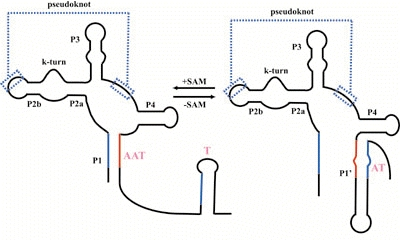
\includegraphics[scale=0.60]{ss-schema}} \hspace{0.05in}
  \subfigure[]{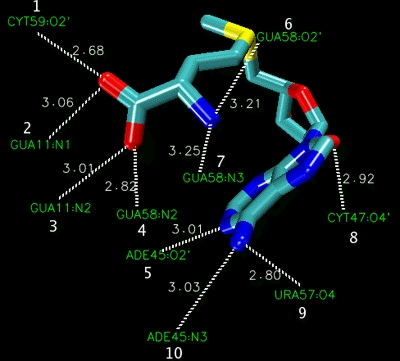
\includegraphics[scale=0.40]{ligand-atom2}}
\caption{Schematic of the secondary structures of s-box riboswitch with SAM bound (left; in the AAT state) and without SAM 
(right; in the AT state); predicted ligand-SAM interactions with s-box}
\end{figure}


\begin{figure}
  \subfigure[]{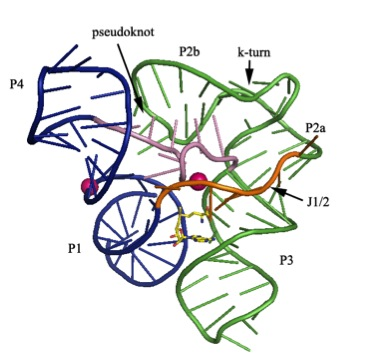
\includegraphics[scale=0.4]{sbox_3D}}
  \subfigure[]{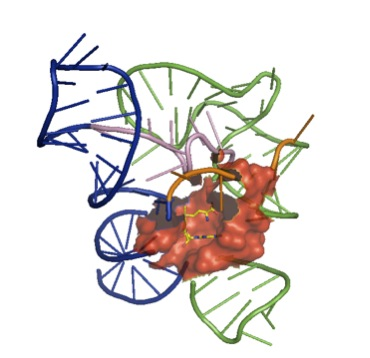
\includegraphics[scale=0.40]{binding_pocket-2}}
  \subfigure[]{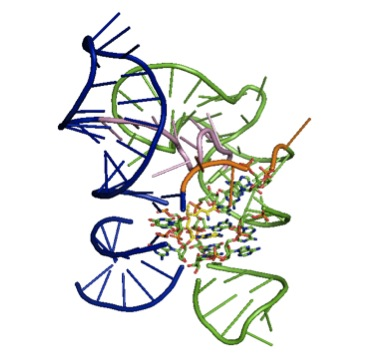
\includegraphics[scale=0.4]{binding_pocket-1}}
\caption{(i) The structure of the S-box riboswitch; (ii) S-box with SAM bound; (iii) Residue number: 7, 11, 
12, 45-47, 57-59, 88, 89}
\end{figure}


\subsubsection*{Initial Results}

Here, we brief MD simulation protocols used for the long time MD simulations of the SAM-I riboswitch.  The starting point of all simulations is the X-ray crystal structure of SAM binding to the AAT conformation of s-box riboswith (PDB: 2GIS)~\cite{montange}. In the simulation of the SAM free s-box riboswitch, SAM is directly removed from the x-ray crystal structure and replaced with solvent water. The amber99bsc0 correction force field is used here~\cite{alberto}. Parameters for SAM are from the Generalized Amber Force Field (GAFF) and missing parameters are calculated using ANTECHAMBER~\cite{wang}. Positions of added hydrogens are guessed using PSFGEN within NAMD 2.6. Then the RNA molecules are solvated in a cubic solvent box of TIP3P waters with a 16A padding in all directions. Sodium and magnesium ions are distributed around the RNA molecules and neutralize charge of the system. The total number of atoms in the system is 56,000. Energy minimizations are carried out on all of the systems to remove bad contacts. Starting from 0 K, the temperature is raised 10 K for every 10,000 steps and is held constant after reaching the desired temperature (310 K) using temperature reassignment. MD simulations are performed in the NPT ensemble with the pressure maintained using the Langevin piston method with a period of 100 fs and decay times of 50 fs. The time step is 2fs for both equilibration and production phase. Bond lengths between hydrogens and heavy atoms are constrained using SHAKE. The long-range electrostatics is treated with the Particle Mesh Ewald (PME) method with a cutoff distance 12A.  All MD simulations are carried out by using a parallel version of NAMD 2.6.  VMD, wordom~\cite{moe} and homemade scripts are employed to analyze the trajectories. All snapshots of structural images are made using VMD.

%All simulations are performed using NAMD 2.6 on LSU (Tezpur) and LONI (Queenbee) Linux clusters. 



\begin{figure}
   \subfigure[]{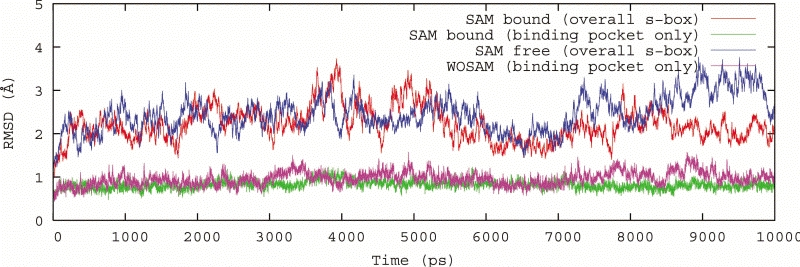
\includegraphics[scale=0.56]{rmsd}} \newline
   \subfigure[]{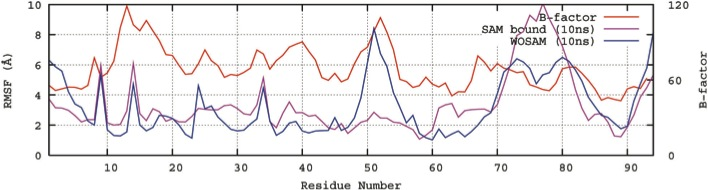
\includegraphics[scale=0.660]{RMSD_residue}}
\caption{RMSD of overall s-box and binding pocket only in SAM bound and WOSAM (short for the 
trajectory of SAM free s-box riboswitch) trajectories  with reference to the crystal structure; (b) Root mean square fluctation (RMSF) and B-factor of each residue of s-box riboswitch from MD trajectories}
\end{figure}

\begin{figure}

   \subfigure[]{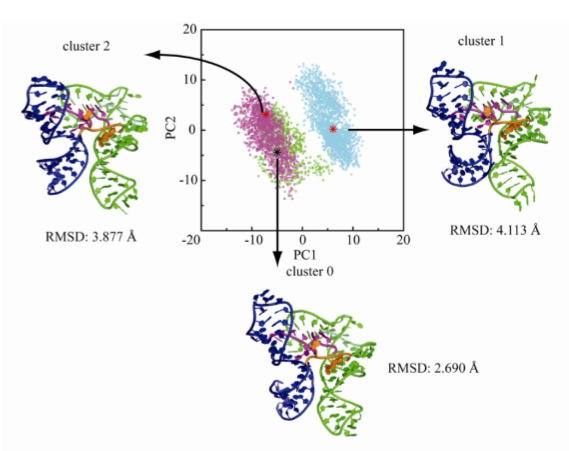
\includegraphics[scale=0.45]{cluster_2D}}
   \subfigure[]{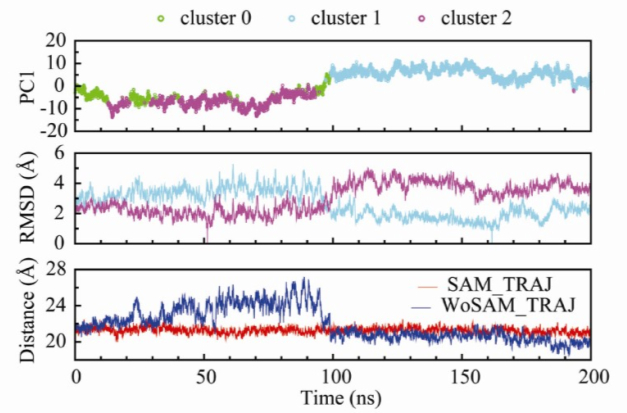
\includegraphics[scale=0.35]{cluster_1D}}

\caption{Clustering and Principal Component Analysis (PCA) point towards a chopstick-like 
motion involving P1 and P3 helices in the absence of SAM. 
(a) Projections of snapshots of the SAM free trajectory are plotted against the first two principal 
components and color coded according to a k=3 k-means clustering: cluster 0: magenta, cluster 1, 
green, cluster 2, magenta. Representative snapshots from each cluster are also shown. This plot 
indicates that snapshots can be broadly clustered into two groups (cluster 1 and cluster 3) with 
cluster 2 representing a group with characteristics similar to those of cluster 3. The projection 
along PC1 broadly separates the clusters, while projection along PC2 completes the separation 
between clusters 1 and 3. Structures of representative snapshots indicate that clusters are 
distinguished by a dramatic change in relative position of P1 and P3. (b) From top to bottom: 
The time evolution of the first principle component of the SAM free trajectory. RMSD for each snapshot in the SAM free relative to the 
representative snapshots for cluster 1 (cyan curve) and for cluster 3 (magenta curve). The 
distance between the Center of Mass (COM) of P1 and P3 for the SAM free trajectory (blue) and for 
the SAM bound trajectory (red).  During the first half of the SAM free trajectory, P1 and P3 helices move apart 
(clusters 0 and 2), then they move back together during the second half of the trajectory (cluster 
1).}

\end{figure}

Our initial achievements are illustrated with novel findings as shown in Figure 5 and Figure 6.  Our results suggest that the presence of SAM in the binding pocket is critical to form P1 helix made of two distal strands.  The essential dynamics found with the SAM-free trajectory are illustrated in Figure 6 with clustering results. 

To estimate the binding affinity, we chose MM-PBSA (Molecular Mechanics - Poisson Boltzmann Surface Area) and initial results indicated that strong electrostatic interactions between SAM and SAM-I as well as the importance of inner-shell bound $Mg^{2+}$ binding  are crucial for the overall SAM binding mechanism.  

%In order to understand the conformational changes and the major dynamical
%modes will require simulations to be to be extended to longer timescale, possibly into hundreds of 
%nanoseconds (we are already touching the limit of 100ns!).
%Specifically we will use the the long-time simulation to explore:

%\begin{itemize}
%\item To find out the collective motion difference between SAM bound and WOSAM, for SAM bound, there 
%may be some collective motion among the binding pocket residues; WOSAM, how the collective motion 
%changes?
%\item Correlation of binding free energy with conformation clusters/PCA analysis
%\end{itemize}

\begin{figure}
   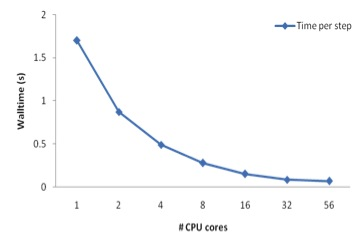
\includegraphics[scale=0.660]{56k_scaling-2}
\caption{Typical wall-clock times taken (in second) for each step at different processor counts.}
\end{figure}


\subsubsection*{Requested computational resources}

In Figure 7, we show the scaling performance with MD simulation package such as NAMD.  When using 32 cores, the time taken per step is approximately 0.06s; thus the wall clock time required to complete 1ns is .34 day; in other words for a 56K system, 1 ns simulations require $\approx$ 300 CPU hours. Thus each 100 ns simulation requires approximately 30,000 CPU hrs. In Table 2, estimated CPU costs are shown.  We expect 750,000 SU are needed for this project.

\begin{table}[!h]
\begin{center}
  \caption{Riboswitch simulations and expected computing resources. Note that the estimated SUs for MM-PBSA calculation is about the additional MD simulation with the SAM-free RNA system}
\label{table:systems}
\begin{tabular}{| c | c | c | c |}
\hline
Molecular System & Type of Calculation &   Method or Package  &   SUs required \\
\hline
SAM-I & MD &  NAMD &  30K\\
SAM-I & MM-PBSA & NAMD & 30K \\
SAM-I & PCA/Clustering &  AMBER and scripts &  50K\\
SAM-II &MD &  NAMD &  15K\\
SAM-II & MM-PBSA & NAMD & 15K \\
SAM-II & PCA/Clustering & AMBER and scripts & 50K \\
SAM-II & REMD &  NAMD &  450K\\
SAM-III &MD &  NAMD &  30K\\
SAM-III & MM-PBSA & NAMD & 30K \\
SAM-III & PCA/Clusetring & AMBER and scripts & 50K \\
\hline
\end{tabular}
\end{center}
\end{table}


\subsection*{Project 3: Expeditions in Distributed Computing using SAGA}

% Although Grid technologies have matured considerably over the past few years, applications that can effectively utilize these technologies are far from ubiquitous.  % Another way in which Grid Application development is being retarded by a lack of suitable abstractions is in the development of ``first principles'' Grid applications -- applications that are able to leverage the heterogeneity and dynamic performance response inherent in the Grid to their advantage -- which have proved exceedingly difficult to implement.

Advances in Grid applications have simply not kept pace with advances in other aspects of distributed cyberinfrastructure, such as Grid middleware -- whether measured by the number of existing applications that can easily utilize the many advanced features offered by distributed infrastructure or measured by the number of novel applications capable of using the infrastructure. A key impediment in the accelerated development and deployment of Grid applications is the scarcity of high-level application programming abstractions that bridges the divide between the needs of Grid applications and the capabilities offered by middleware.  Much Grid development has focused on the support for legacy parallel and cluster applications codes as a way of ensuring scientific relevance.  The benefit of the Grid paradigm, however, will come from new application development that does not depend on the homogeneous and relatively static model of resource performance inherited from parallel or cluster legacies.  The lack of such application-level programming abstractions is compounded by the fact that there exist incompatible and often changing Grid middleware systems in both research and production environments.  To address these challenges and in particular to find a solution to the universal, apparently intractable problem of successfully Grid-enabling applications, several applications groups expressed the desire for a simple programmatic interface that is widely-adopted, usable and available.  The goal of such an interface would be to provide a ``grid counterpart to MPI'' (at least in impact if not in details) and that would supply developers with a simple, uniform, and standard programmatic interface with which to develop distributed applications.  Thanks to the efforts of many contributors, an initial specification of such a ``grid counterpart to MPI'' now exists -- the Simple API for Grid Applications (SAGA). As of early 2008, SAGA is now an Open Grid Forum (OGF) technical recommendation.

% SAGA has the following properties:

% \begin{itemize}
% \item Simplicity: easy to use, install, administer and maintain
% \item Uniformity: provides support for different application programming languages as well as consistent 
% semantics and style for different Grid functionality
% \item Scalability: Contains mechanisms for the same application (source) code to run on a variety of 
% systems ranging from laptops to HPC resourcesGenericity: adds support for different grid middleware, 
% even concurrent ones
% \item Modularity: provides a framework that can be easily extended to incorporate new functional areas
% \end{itemize}


\subsubsection*{Developing and Deploying Applications using SAGA}

% It is important to note that the SAGA effort is a world-wide effort that is {\bf led} by as well as coordinated by our group at the CCT~\cite{saga_url} -- from the specification and standardization process, to the implementation and development of the appropriate adaptors.  Even as the SAGA standad has evolved, its C++ implementation and complete adaptor sets are being developed, we have been developing applications that utilise SAGA to facilitate the use of distributed resources.  
A wide range of applications have been developed -- ranging from regular compute intensive applications but involving multiple resources ~\cite{saga_escience07}, applications with irregular compute resources ~\cite{teragrid08} as well data-intensive applications ~\cite{sagamapreduce} using programming abstractions such as MapReduce~\footnote{Implementation of MapReduce using SAGA is funded by Google} An initial prototype of a ``general pilot-job'' framework using SAGA that can be utilized for Replica-Exchange that enables the {\it trivial} utilisation of multiple distributed resources across LONI and now Teragrid has been developed. This is currently work in progress, but we anticipate sufficient progress to begin testing the framework using our 56K riboswitch model.~\cite{REMD-PhilTranA2009}. ABrief schematic of Distributed Adapative Replica Exchange Molecular Dynamics is shown in Figure 9.  Our current framework implements the glide-in feature with the BigJob abstraction built upon SAGA and utilization of the framework is the key component for successful massive REMD simulations for our project on riboswitch studies.

%and soon to be specific biomedical applications (using ParaMedic, for which the PI along with others was awarded the Best Paper award at the International SuperComputing Conference held in Dresden in June 2008). Of particular interest to the Biomolecular simulation community (within LONI and Cybertools project) is our effort to develop a


\begin{figure}
\begin{center}
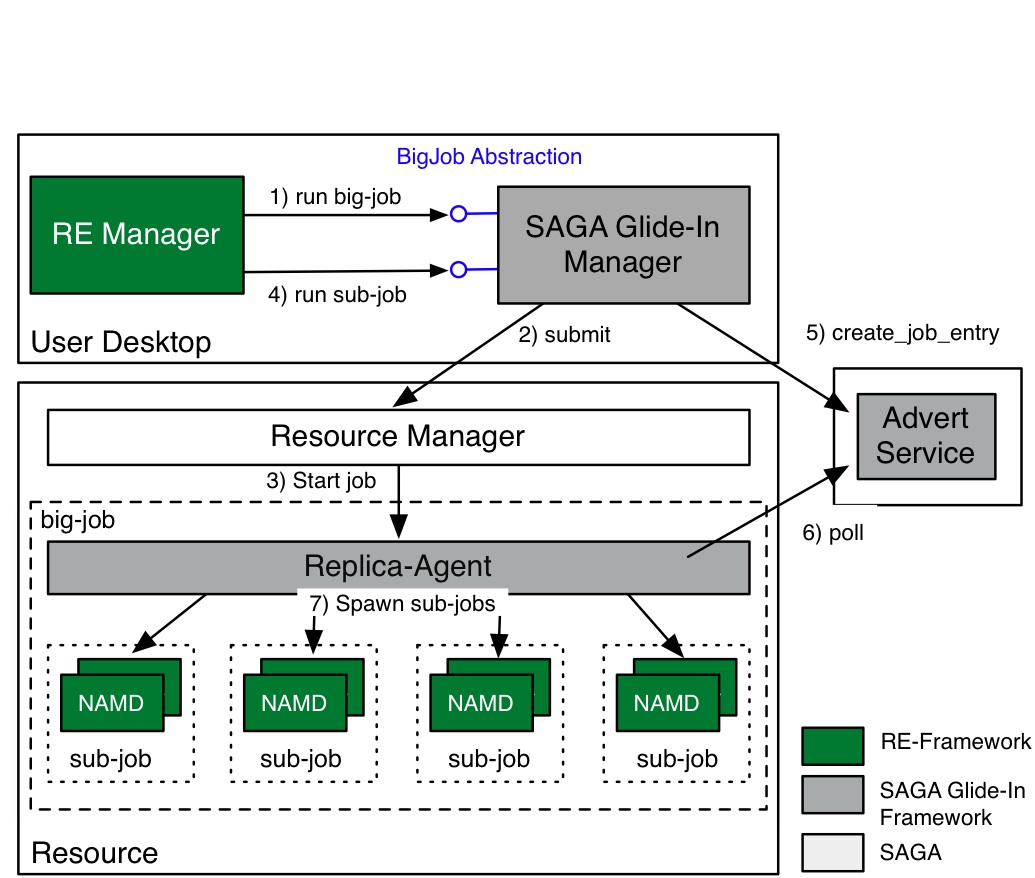
\includegraphics[scale=0.65]{DARE-MD}
\end{center}
\caption{Schematic of Distributed Adaptive Replica Exchange framework using the BigJob abstraction that is built upon SAGA.}
\label{fig:results}
\end{figure}

\subsubsection*{Developing Autonomic Computing Frameworks for CO$_2$ Sequestration Studies using SAGA}

Global energy needs today present serious challenges: the increasing demand for energy must be met, however at the same time the emissions of greenhouse gases into the atmosphere must be reduced. Even as alternative energy sources continue to develop and gain popularity, the fact remains that fossil carbon resources will continue to be in heavy use (in both developing and industrialized countries) and consequently generate large volumes of carbon dioxide ~\cite{GeoRPT}. The atmospheric impact of this greenhouse gas can be abated through capturing and sequestering significant fractions of the produced CO$_2$.

For long-term storage of large volumes of CO$_2$, porous subsurface geologic formations are ideal candidates: these are the same formations responsible for the existence of oil and gas reservoirs. Indeed much the technology behind carbon dioxide sequestration (including drilling, gas injection, reservoir management and of course reservoir simulation) stems from drilling, petroleum and reservoir engineering. Injecting CO$_2$ into an oil-gas reservoir can also lead to improved oil recovery by ``pushing out'' the oil and gas for production, this allows for reduced net cost through increased revenues from oil and gas production ~\cite{EORBook}.

\begin{figure}
\begin{center}
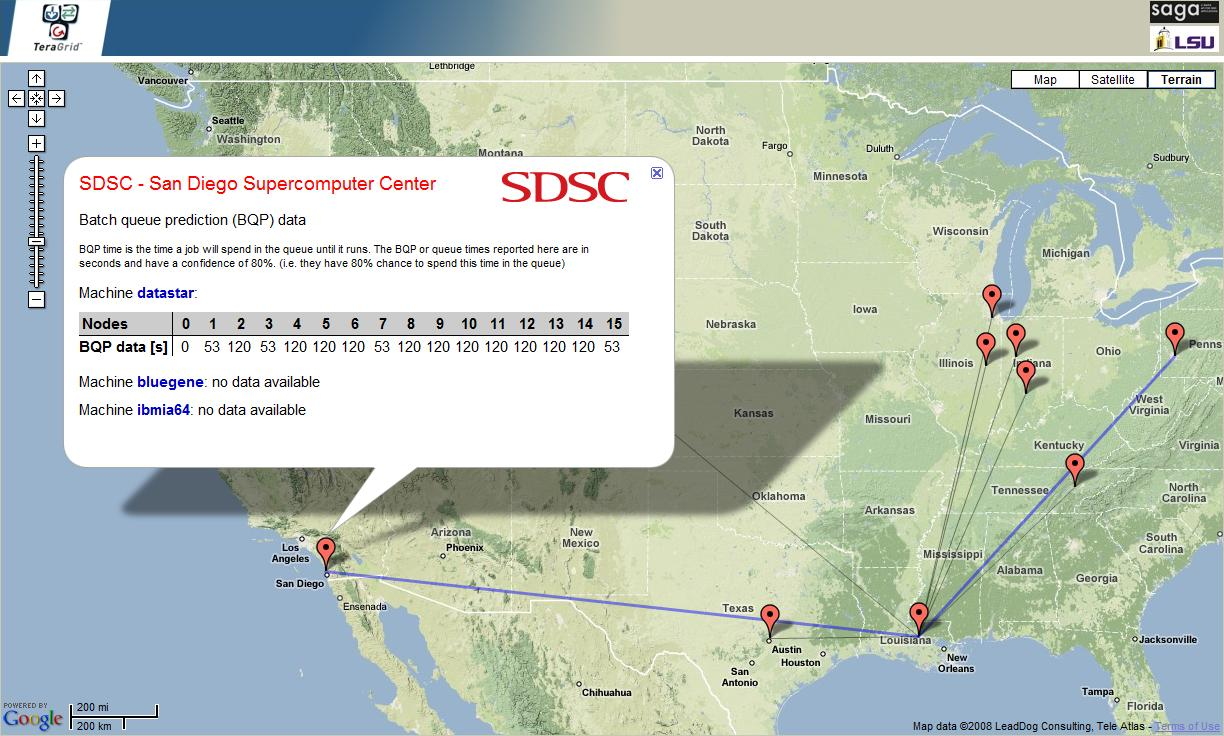
\includegraphics[scale=0.33]{gmaps_bqp.jpg}
\end{center}
\caption{A snapshot of an application using batch-queue-prediction system to dynamically determine the best resource to spawn a sub-task to; the noteworthy point is that the entire decision process is at the application level -- the fact that the applicaiton has to spawn a job of requirements X is mapped to a reource requirements, BQP is used to determine the resource based upon optimal availablity and then the application uses SAGA to spawn and launch the sub-task onto the chose resource. A paper demonstrating this feature working across the TeraGrid won the Performance Challenge Award at TeraGrid 2008 (Ref.~\cite{teragrid08})}
\label{}
\end{figure}

One of the major areas of research in this field is the characterization of reservoirs that are safe and secure, environmentally and geologically and are therefore promising candidates for CO$_2$ sequestration ~\cite{GeoRPT,Luigi}. Our efforts are directed towards developing cyberinfrastructure tools, technologies and abstractions that facilitate large scale reservoir characterization and forecasting studies.

Since the amount of information obtained directly from reservoirs is very small compared to the actual size of the reservoir, history matching techniques have been developed to match actual reservoir production with simulated reservoir production, therefore obtaining a more ``satisfactory'' set of reservoir models. One of the promising approaches to history matching is the use of Ensemble Kalman filters (EnKF) ~\cite{KalmanPaper, DO2007, LiEnKF07, DO2006}.

Ensemble Kalman filters are recursive filters that can be used to handle large, noisy data; the data in this case would be the results and parameters from ensembles of reservoir models that are sent through the filter to obtain the ``true state'' of the data. Since the reservoir model varies from one ensemble to another, the run-time characteristics of the ensemble simulation are irregular and hard to predict. Furthermore, at simulation times when real historical data is available, all the data from the different ensembles at that simulation time must be compared to the actual production data, before the simulations are allowed to proceed. This translates into a global synchronization point for all ensembles; hence performing large scale studies for complex reservoirs in a reasonable amount of time would benefit greatly from the use of distributed, high performance, high throughput and on-demand computing resources.

\begin{figure}
\begin{center}
\includegraphics*[scale=0.4,angle=0]{3StageKalmanFilter}
\end{center}
\caption{Schematic illustrating the variability between stages of a typical
  ensemble Kalman filter based simulation. The end-to-end
  application consists of several stages; in general at each stage the
  number of models generated varies in size and duration.}
\label{fig:irregular_execution}
\end{figure}

To this end we developed several components: a CO$_2$ sequestration simulator and an autonomic, self-monitoring, self healing and self optimizing job management framework: the Lazarus framework ~\cite{gmac}. Early investigation of the {\it Scale-Out} performance of Lazarus on single and distributed TeraGrid resources are promising, with a significantly reduced total time to completion in the optimized, distributed cases.

\begin{figure}
\begin{center}
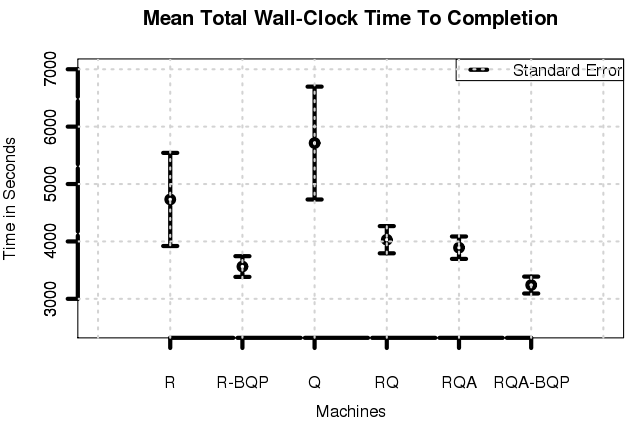
\includegraphics[scale=0.8]{Figure7.png}
\end{center}
\caption{Demonstrating the effectiveness of Distributed Applications Developed  Using SAGA to Scale-Out. From Left to Right, Performance as measured by the time-to-completeness of a well-defined workload when using: (i) Ranger only (ii) Ranger (with BQP service) only, (iii) QueenBee only, (iii) Ranger and QueenBee, (iv) Ranger, QueenBee and Abe concurrently (v) Ranger, QueenBee 
  and Abe when using BQP service. From Ref.~\cite{gmac} }
\label{fig:results}
\end{figure}

\subsubsection*{Utilizing Application-level Interoperability across TeraGrid and DEISA}
As part of NSF funded HPCOPS Award, LONI has begun a year long project to utilize the aggregated computational power of the Federated Grids of DEISA and TeraGrid. The aim of the project is to (i) work towards an integrated infrastructure that supports application level-interoperability and, (ii) having created the infrastructure apply it to the scientific problem of understanding the conformational challenges and determining the free energy...

\jhanote{Provide URL of the project. Mention its funded. Mention Project
has guaranteed resources from the UK NGS and DEISA. Need approximately
500K Roaming across, QB/Abe, Kraken, Ranger}


% A major limitation we are facing at the moment is the fact the allocations currently used in the group are small and limited to a few machines, forcing us to reserve the allocations for production runs and not benchmarks or development runs.

{\it Roaming Resource:} To state the obvious, if a primary aim of our work is to investigate the ability of distributed applications to {\it Scale-Out}, then it is imperative that there be an underlying resource allocation to support the work. We aim to develop frameworks such as Lazarus and Faust to support the ability of applications to {\it Scale-Out} in a manner that is independent of the specifics of the applications.

%  This hinders our capacity to perform full scale testing of Lazarus' {\it Scale-Out} to the intended target of at least one million simulations.

{\it Resource Requirements:} For Project 3, we require 250,000 SUs; this is the more experimental component of this proposal, where we do not have clear estimates and benchmarking data. However, based upon our experience/publications alluded to in the previous paragraph, each "experiment" that we conduct, (ie application that we develop), requires a minimum of 50000 SUs. For example, running a reservoir simulation for a simulation
time of two weeks (typical period of historical production data gathering) consumes about ten minutes on four cores. 
With two hundred ensembles (typical number of ensembles), running for a simulation time of fifteen years will consume
48k SUs. This obviously is the medium range of simulations; a more detailed reservoir model
will naturally consume more SUs per simulation, multiplied by a large number of ensembles and the SUs required
to perform the history matching increases dramatically. To complete the forecast stage, we will need to run
the same ensembles for an extended period of time (reservoir depletion/workover, enhanced oil recovery and
CO$_2$ sequestration) which roughly would range between twenty to thirty years in simulation time, that is
an additional 64k-96k SUs, placing the total in the range of 112k-144k SUs for a single complete reservoir study.

\begin{table}[!h]
\begin{center}
 \caption{Summary of allocation usage for a typical simulation}
\begin{tabular}{| c | c |}
\hline
Simulation Time & 0.041667 years \\ 
\hline
SU cost per Simulation & 0.6667 SUs \\ 
\hline
Target History Matching Simulation Time & 15 years \\ 
\hline
Target Forecast Simulation Time & 20 years \\ 
\hline
Number of Simulations & 200 \\ 
\hline
Total Cost in SUs & 112k\\
\hline
\end{tabular}
\end{center}
\end{table}


{\it Supporting Grants:} This work is funded by the UCoMS project, Department of Energy and Louisiana Board of Regents
award No. DE-FG02- 04ER46136 

The PI leads Work Package 4 of the NSF Funded Cybertools Project
(http://www.cybertools.org) (NSF Award Number-00000, Total Value
\$12M).

PI-Jha is also the co-PI of LSU/LONI's HPCOPS NSF award, ``Joining the TeraGrid'', member of the Scientific Board of the LONI Institute.  Project 2 is funded by multiple Louisiana Board of Regents award and an LSU Faculty Award (PI Jha). Integration of SAGA with applications is part of Cybertools and the PI also holds multiple peer-reviewed awards for the development and integration of SAGA.

Current the ``


{\it TeraGrid User Support:} Since our applications have been developed, tested and benchmarked on the TeraGrid resources
we are requesting allocations on, we do not foresee any need for support from TeraGrid personnel.

\bibliographystyle{unsrt}
\bibliography{jha_loni_alloc_jul01}



%\subsection*{Project 1: Nucleic Acid Translocation through Alpha-Hemolysic Protein Nanopore}

%Translocation of nucleic acid strands through confined protein pores has biological relevance in instances 
%such as viral transfer of genetic material across a membrane.
%Nanopore current recording experiments can reveal information on a polymer translocating through a pore 
%such as the well characterised protein pore $\alpha$-Hemolysin (Fig.1). A nanopore is inserted into a lipid 
%bilayer and a transmembrane potential is applied. The ionic current through the pore is measured and the 
%translocation of polymers through the pore causes a measurable current blockade by obstructing the flow 
%of electrolytes through the pore.
%With high enough output resolution, the sequence of a DNA strand could be attained. By simulating the 
%translocation event, our understanding of the microscopic processes involved will increase. This could 
%move the field towards genetic sequencing.

%The high-level scientific objective for this project is to compute the free energy
%profile of the translocation process of DNA along the vertical axis of a a
%transmembrane protein pore buried in a lipid membrane bilayer. This is a project that has been ongoing for nearly two years (which was 
%initiated before my transition to LSU),  has consumed a total of $\approx$ 1.5M SUs
%so far (of which 200,000 are on LONI) and we are now very close to 
%major publication in a high-profile journal (Fall 2008). 
%Over the past 24 months, we have been performing an extensive series of
%simulations of DNA translocation through the $\alpha$-hemolysin nanopore by a
%novel combination of algorithm and computational infrastructure. The possible
%parameter space of the problem that needs to be explored is huge, but through
%our studies we have
%determined the optimal values at which to perform the non-equilibrium simulations.
%%simulations. This work follows as a natural extension of the work done as part
%%of the SPICE project which won the HPC Analytics Challenge Award at
%%SuperComputing'05 and the Life Science Award at International Supercomputing
%%Conference 2006. 
%The project uses the parallel MD code NAMD and as also led to a 
%grid-enabled version of NAMD developed by us to perform steered MD simulations
%including the capability to connect to distributed haptic devices. This work is currently 
%funded by the UK's EPSRC (equivalent to the US NSF).
%Current and near-future
%work, also forms the basis of a joint US-UK submission to the NSF (in collaboration 
%with Prof.'s Zuzanna Siwy (UC-Irvine) and Stefan Howorka (London)). 

%{\bf Principal scientific objectives:} To compute the free
%energy profile of the translocation process of DNA along the vertical axis of
%a transmembrane protein pore buried in a lipid membrane bilayer.  There are
%presently established methods of experimentally deducing the base sequence of
%nucleic acid chains, however, such methods are not economically accessible
%enough to allow for the decoding of DNA for purposes such as in medical
%analysis. As Akeson~\cite{akeson} have shown, threading nucleic acid chains through
%transmembrane porous proteins (such as $\alpha$-hemolysin) in a single channel
%current recording apparatus can provide information indicating sequence. At
%the resolution of the data retrieved from the experiments of Akeson,
%conclusions were limited, not allowing the differentiation of individual
%bases. It is proposed that steps towards individual base coding by this method
%can be made by increasing the translocation time of nucleic acid chains
%through the pore, or making the extent of blockage more distinct based on the
%type of base. This can be achieved either by chemical modification of the pore
%surface or modification of the nucleic acid chain itself, yielding a higher
%resolution current readout. Experimentally, Akeson showed that threading
%single-stranded dA and dC based nucleic acid chains results in different
%translocation times and different degrees of pore blocking. To understand
%experimental results and explore alterations to this method, computer
%simulations can be performed that compute the free energy profile of the
%various ssDNA sequences that translocate and thus provide the required insight
%into the physical mechanisms responsible for the significant change in the
%translocation time. Using NAMD our simulations  mimic - in a 'natural'
%environment - the translocation process. 

%We use constant velocity Steered Molecular Dynamics (cv-SMD) is used to reduce simulation computation to practical levels. In cv-SMD, fast translocation is performed by pulling the front most residue of a single stranded DNA strand at constant velocity.  The equilibrium free energy profile is extracted from the non-equilibrium work done using Jarzynski�s Equality~\cite{jarz}.
%In addition to verifying the experimental results (which should be amenable to
%relatively small scale simulations), moving 20-base long single-stranded A and
%dC nucleic acid chains inside the protein pore and analysing differences in
%the free energy profile/work done in the process, will test the ability of our
%method to distinguish difference sequences.
%The ability to compute via simulations, the 
%free energy profiles along sub-sections of the pore has immediate consequences for
%DNA sequencing.

%%Following that we would also
%%like to simulate the movements of longer chains of 50-base length (of both dA
%%and dC) in order to explore the effect that the length of the DNA strand has
%%on the profile(s).

%\begin{figure}
%\begin{center}
%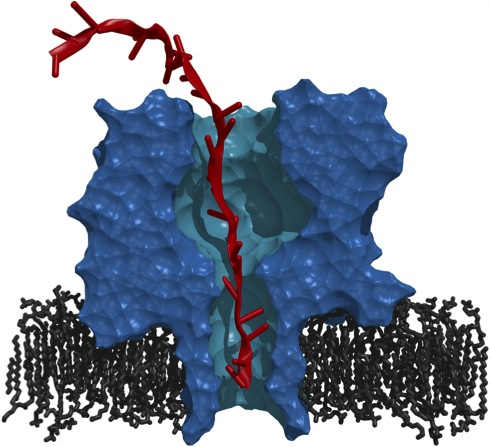
\includegraphics[scale=0.5]{pore_dna-1.jpg}
%\end{center}
%\caption{Single stranded DNA translocation through $\alpha$-Hemolysin. A cross-section of the protein 
%pore $\alpha$-Hemolysin is depicted in blue. Red represents a single strand of DNA (3 end at the bottom).  
%Black represents the lipid bilayer.  The DNA strand is translocted from the cis (top) entrance to the trans 
%(bottom) entrance.}
%\label{}
%\end{figure}

%\begin{figure}
%  \subfigure[]{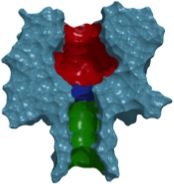
\includegraphics[scale=0.750]{pore_structure-1}}  \hspace{1.5in}
%  \subfigure[]{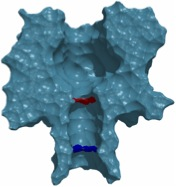
\includegraphics[scale=0.750]{pore_structure-2}}
%\caption{These simulations are concerned with translocation at the constriction (blue) and beta barrel 
%(green) of $\alpha$-HL. Red represents the alpha chamber.
%Here the translocation resistance is highest due to the pore dimensions.
%Key pore residues present themselves when pulling poly-Adenine across this region at 0.004 A/ps. 
%Methionine residue 113 (red) and Leucine residue 135 (blue) show peaks in work profile.}
% \label{model}
%\end{figure}

%\begin{figure}
%  \subfigure[]{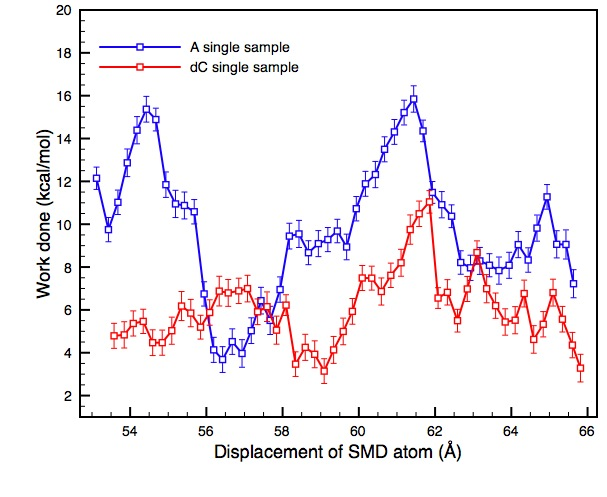
\includegraphics[scale=0.4]{single_sample_A_vs_dC_135}}  
%  \subfigure[]{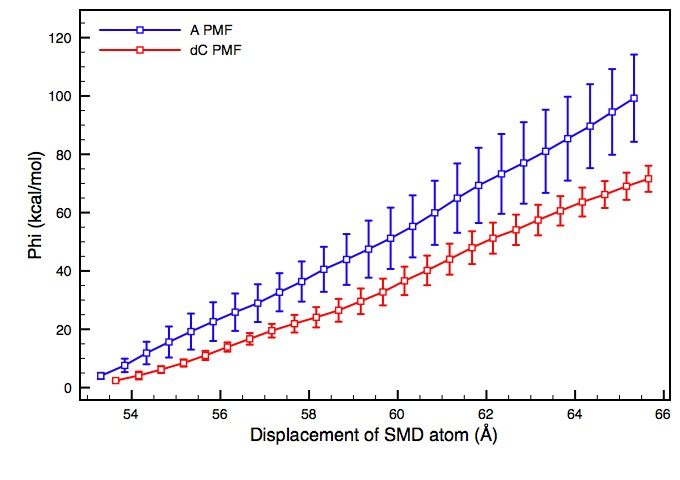
\includegraphics[scale=0.4]{dC_vs_A_PMF}}
%\caption{Simulation results show the difference in the work profile of translocation between nucleotide
%chains with differing secondary structure (A vs dC). The figure to the left is for a single sample -- local
%energetic profiles, which is capable of distinguishing the main features and events contributing to the profile.
%The figure to the left is the total work profile over the complete pore, averaged over several samples (six in 
%this case). There are indications that the total translocation work energy distinction between A and dC lies 
%well beyond the error bars.}
% \label{model}
%\end{figure}

%

%\begin{figure}
%\begin{center}
%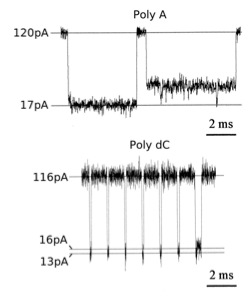
\includegraphics[scale=0.60]{polyA_polydC.jpg}
%\end{center}
%\caption{Single molecule current traces for poly Adenine and poly-deoxy-Cytosine2.
%Poly-A takes ~20 times longer to translocate than poly-dC.
%; experimental evidence of different translocation times for oligo-nucleotide chains
%of A and dC (differing in secondary structure); the precise mechanism of this
%difference is not understood by experiments; our computer simulations provide
%inside in to the different "dwell" times.}
%\label{}
%\end{figure}

%
%{\bf Resources Requested:}

%The code we use is NAMD - a well established, community code that has been
%extensively validated and tested for scalability (for more
%benchmark/performance data, see:
%http://www.ks.uiuc.edu/Research/namd/performance.html). Timings for our system
%(approximately 320,000 atoms) as benchmarked are: \\
%%1.30 days/ns on 64 cores, 0.60 days/ns on 128 cores, 0.35 days/ns on 256 cores.
%Back when queen bee was running slower~\footnote{we helped diagnose
%a hardware problem with Queen Bee} and we were using 384 processors: \\ % \newline
%  \indent performance on 384 CPUs 0.0529952 s/step (0.306685 days/ns) \newline
%Now it's faster and we are using 256 processors the performance is: \newline
%  \indent on 256 CPUs : 0.0506383 s/step (0.293045 days/ns)  \footnote{with similar performance on Tezpur}

%Thus, simulations of our systems are most efficient on 256 cores (consistent with the NAMD rule-of-thumb of approximately 1000 atoms per core), and it
%takes approximately 2000 CPU hrs to simulate one nanosecond. 
%Thus, at a optimal pulling speed, (as there is a compromise between statistical and systematic errors),  it takes the equivalent of $\approx$ 5ns of simulation time for the ssDNA to be pulled through the relevant and interesting portion of the pore. Given that these are non-equilibrium
%simulations, based upon our experience from the SPICE project~\footnote{see http://www.realitygrid.org/Spice and publications therein}, we need 
%on average 8-12 simulations to get a measure of the free energy profile.  Taking
%10 as the typical number of samples required, we need 10 x 5 x 2000 = 100000 CPU hrs, to
%gather enough statistics for a single  translocation study (for example, a
%specific nucleotide sequence and length).
%A single translocation study represents just the beginning of many simulations that will be needed to explore
%the (rich) phase-space of this problem in order to understand the physical
%properties of this important system and the specific science problems.
%Specifically, the science problems that we are addressing are:
%\begin{itemize}
%\item Effect of secondary structure on the translocation times
%\item  Exploring specific interactions that are the dominant component
%of the "dwell" time within the pore
%\item Understanding the difference between the translocation properties
%of a single nucleotide versus a 20-mer oligo-nucleotide, so as to 
%be able to discern the "single" compoent in the "extended, collective"
%dynamics of longer polymer chains
%\item Mutation studies need to be performed to help distinguish steric interactions from other (e.g.,
%hydrophobic) interactions
%\end{itemize}

%The fundamental computational challenge arises from the requirement to perform
%a multiple number (between 8-12) of samples of the same "pulling event"; this is
%a consequence of the non-equilibrium simulations/methods and thus the stochastic nature of the simulations. However, in spite of this, the method used 
%is still at least an order of magnitude quicker than "slow motion" real dynamics MD simulations.

%We anticipate being able to make progress on items 1 (and related to it item 2)
%and item 5; this is what we anticipate we will be able to achieve over the next six months. 
%For each item, we anticipate a lower bound of 200,000 SUs; thus we are requesting
%400,000 SU hours for project I. We will be back 
%with a request for more hours if we were to effectively study the different specific
%science objectives.






\end{document}



